\begin{figure}[H]
  \centering
  \begin{subfigure}[b]{\textwidth}
    \centering
    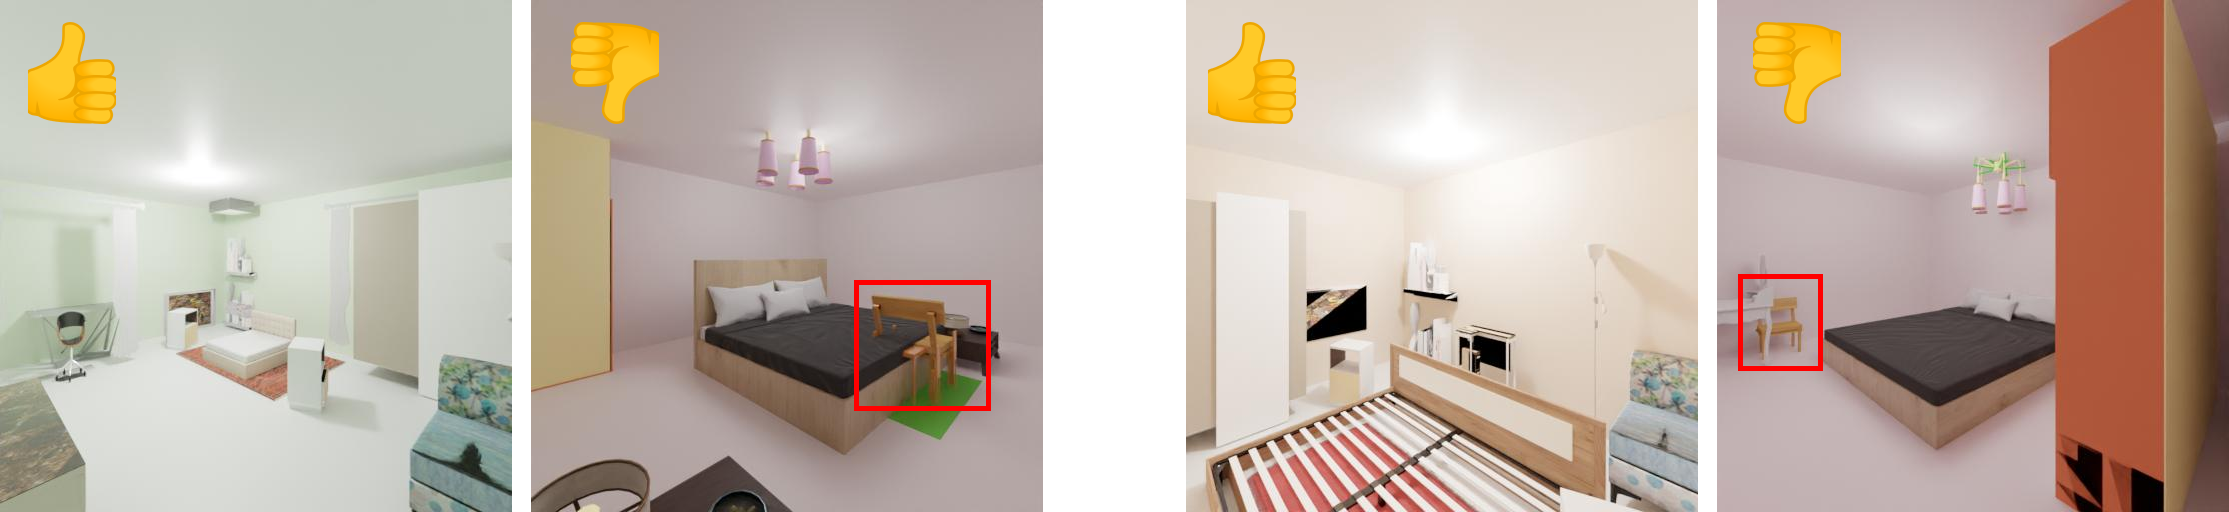
\includegraphics[width=\textwidth,height=\textheight, keepaspectratio]{images/ValidationQuestionBed.png}
    \caption{Bedroom Control Scenes}
    \label{fig:userstudybed}
  \end{subfigure}
  \hfill
  \begin{subfigure}[b]{\textwidth}
    \centering
    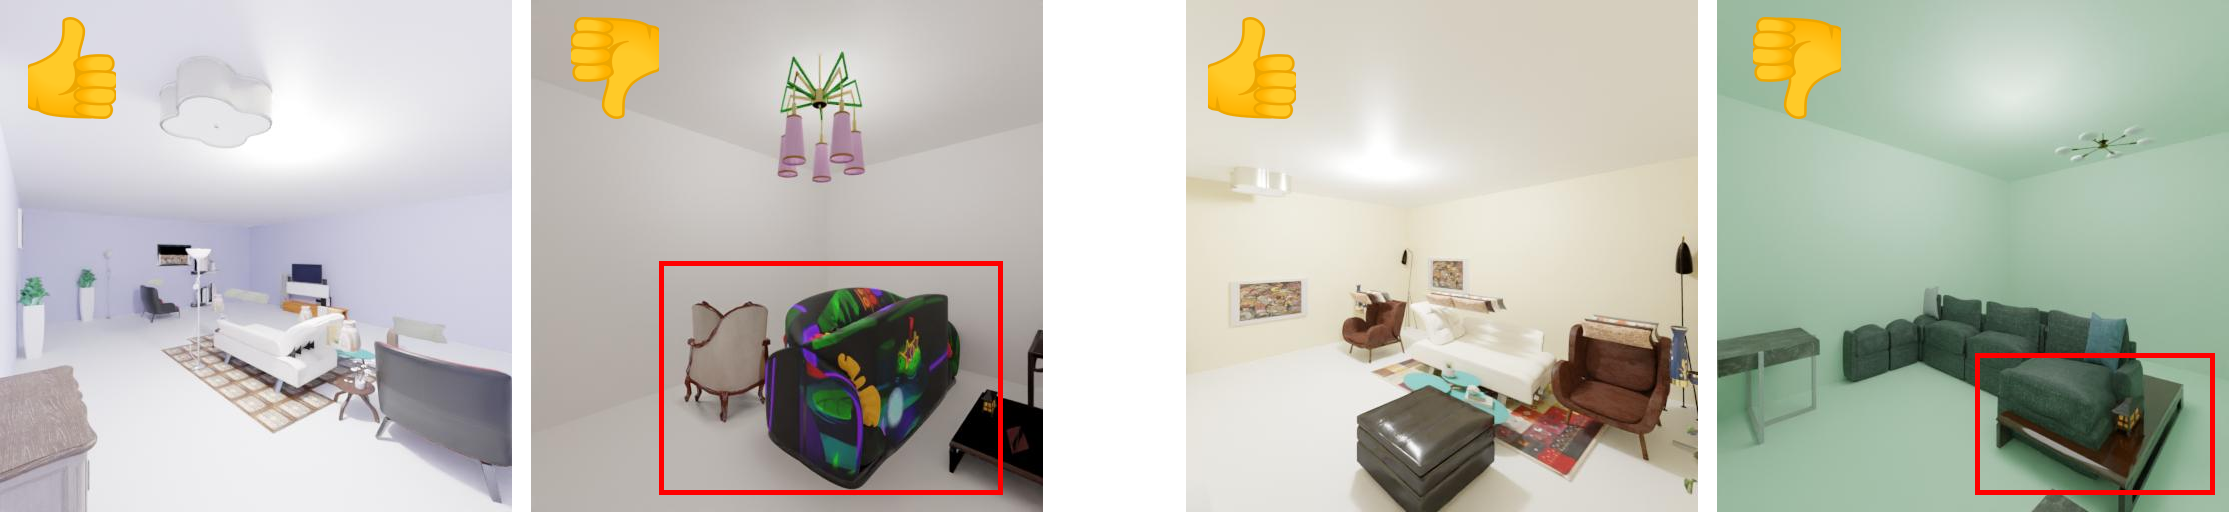
\includegraphics[width=\textwidth,height=\textheight, keepaspectratio]{images/ValidationQuestionLiv.png}
    \caption{Living Room Control Scenes}
    \label{fig:userstudyliv}
  \end{subfigure}
  \caption{
    \textbf{Control Questions for the Subjective Study}
    Here are two control questions provided for our subjective study focusing on bedrooms in Figure \ref{fig:userstudybed} and living rooms in Figure \ref{fig:userstudyliv}. These questions are designed to prompt participants to assess object collisions and the level of detail present in the scenes. The red boxes show the object collisions in the scenes.
    }
\end{figure}